\documentclass{beamer}

\usefonttheme{professionalfonts} % using non standard fonts for beamer
\usefonttheme{serif} % default family is serif

\usepackage{hyperref}

%\usepackage{minted}

\usepackage{animate}

\usepackage{graphicx}

\def\Put(#1,#2)#3{\leavevmode\makebox(0,0){\put(#1,#2){#3}}}

\usepackage{color}

\usepackage{tikz}

\usepackage{amssymb}

\usepackage{enumerate}


\newcommand\blfootnote[1]{%

  \begingroup

  \renewcommand\thefootnote{}\footnote{#1}%

  \addtocounter{footnote}{-1}%

  \endgroup

}

\makeatletter

%%%%%%%%%%%%%%%%%%%%%%%%%%%%%% Textclass specific LaTeX commands.

 % this default might be overridden by plain title style

 \newcommand\makebeamertitle{\frame{\maketitle}}%

 % (ERT) argument for the TOC

 \AtBeginDocument{%

   \let\origtableofcontents=\tableofcontents

   \def\tableofcontents{\@ifnextchar[{\origtableofcontents}{\gobbletableofcontents}}

   \def\gobbletableofcontents#1{\origtableofcontents}

 }

%%%%%%%%%%%%%%%%%%%%%%%%%%%%%% User specified LaTeX commands.

\usetheme{Malmoe}

% or ...

\useoutertheme{infolines}

\addtobeamertemplate{headline}{}{\vskip2pt}



\setbeamercovered{transparent}

% or whatever (possibly just delete it)

\makeatother

\begin{document}
\title[DCEL proposal]{A Parallel DCEL Proposal}
\author[AC]{Andres Calderon}
\institute[Summer'19]{University of California, Riverside}
\makebeamertitle
\newif\iflattersubsect

\AtBeginSection[] {
    \begin{frame}<beamer>
    \frametitle{Outline} 
    \tableofcontents[currentsection]  
    \end{frame}
    \lattersubsectfalse
}

\AtBeginSubsection[] {
    \begin{frame}<beamer>
    \frametitle{Outline} 
    \tableofcontents[currentsubsection]  
    \end{frame}
}

\section{DCEL basic concepts}

\begin{frame}{What is a DCEL?}
    \begin{itemize}
        \item Doubly connected edge list (DCEL) is a data structure suited to represent a connected planar graph embedded in the plane (Muller-Preparata, 2017).
        \item A planar embedding of $G = (V, E)$ does not allow crossing edges.
        \item DCEL captures key topological information about \textbf{vertices}, \textbf{edges }and \textbf{faces}.
    \end{itemize}
%    \centering 
%    \includegraphics[width=.7\linewidth]{p1.png} 
\end{frame}

\begin{frame}{DCEL examples}
    \centering 
    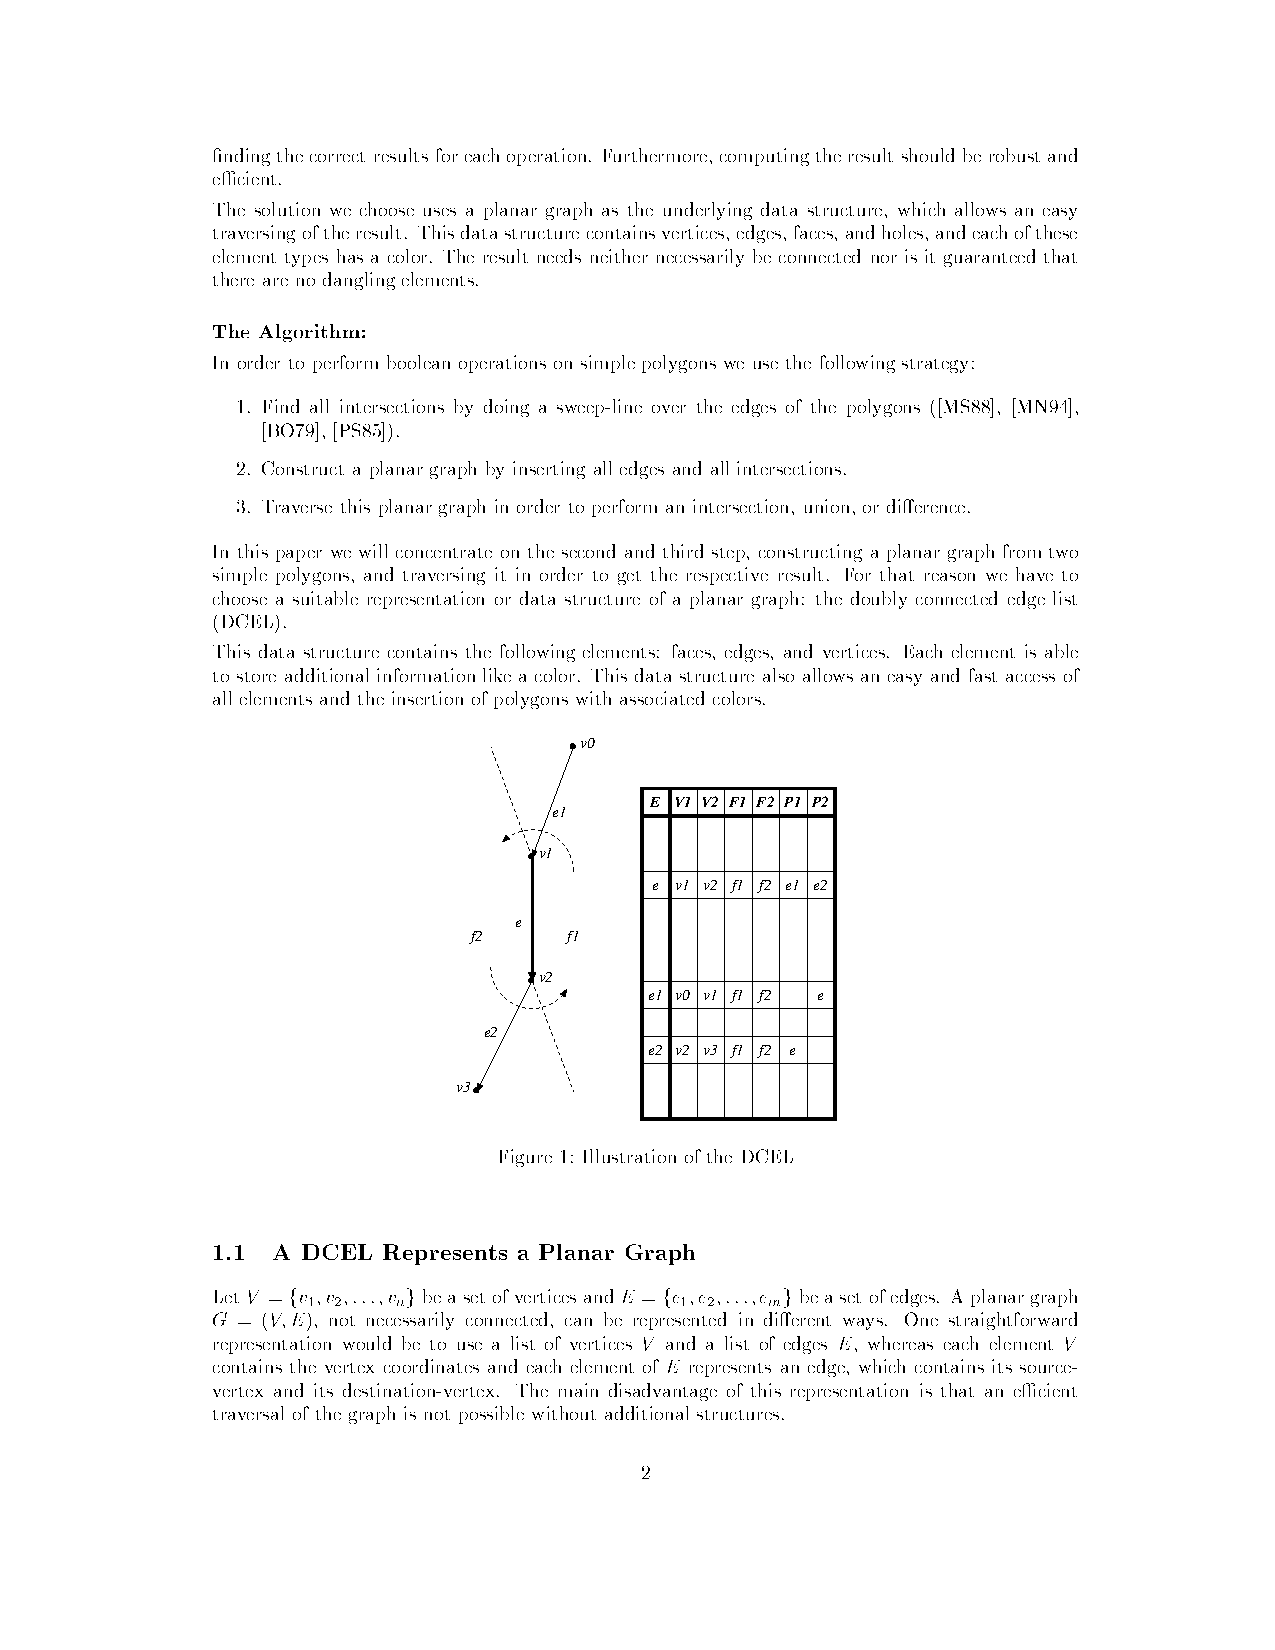
\includegraphics[clip, trim=5cm 9cm 5cm 13cm,width=\linewidth]{figures/dcel01} 
    \flushright \tiny (Freiseisen, 1998)
\end{frame}

\begin{frame}{DCEL examples}
    \centering 
    \begin{minipage}[t]{0.45\textwidth}
        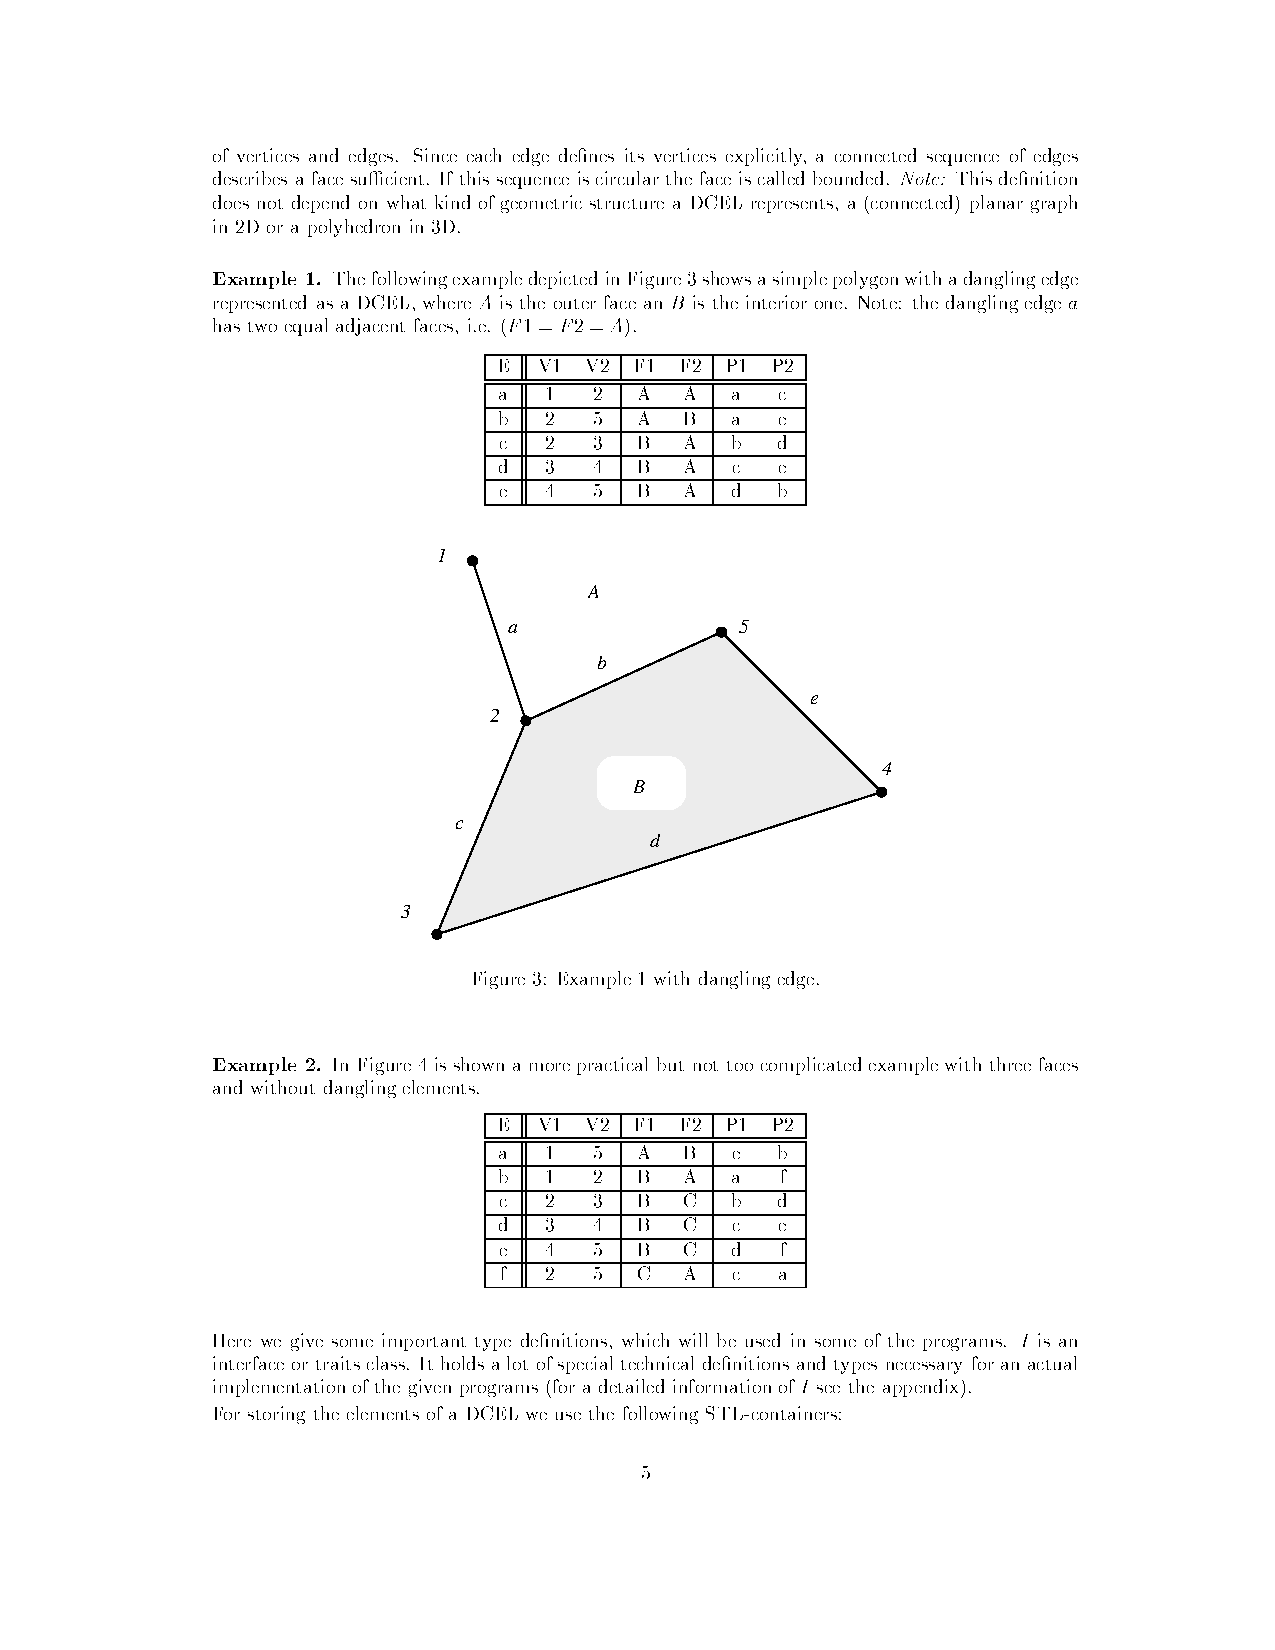
\includegraphics[clip, trim=7cm 12cm 6cm 9cm,width=\linewidth]{figures/dcel02} 
    \end{minipage}
    \begin{minipage}[t]{0.45\textwidth}
        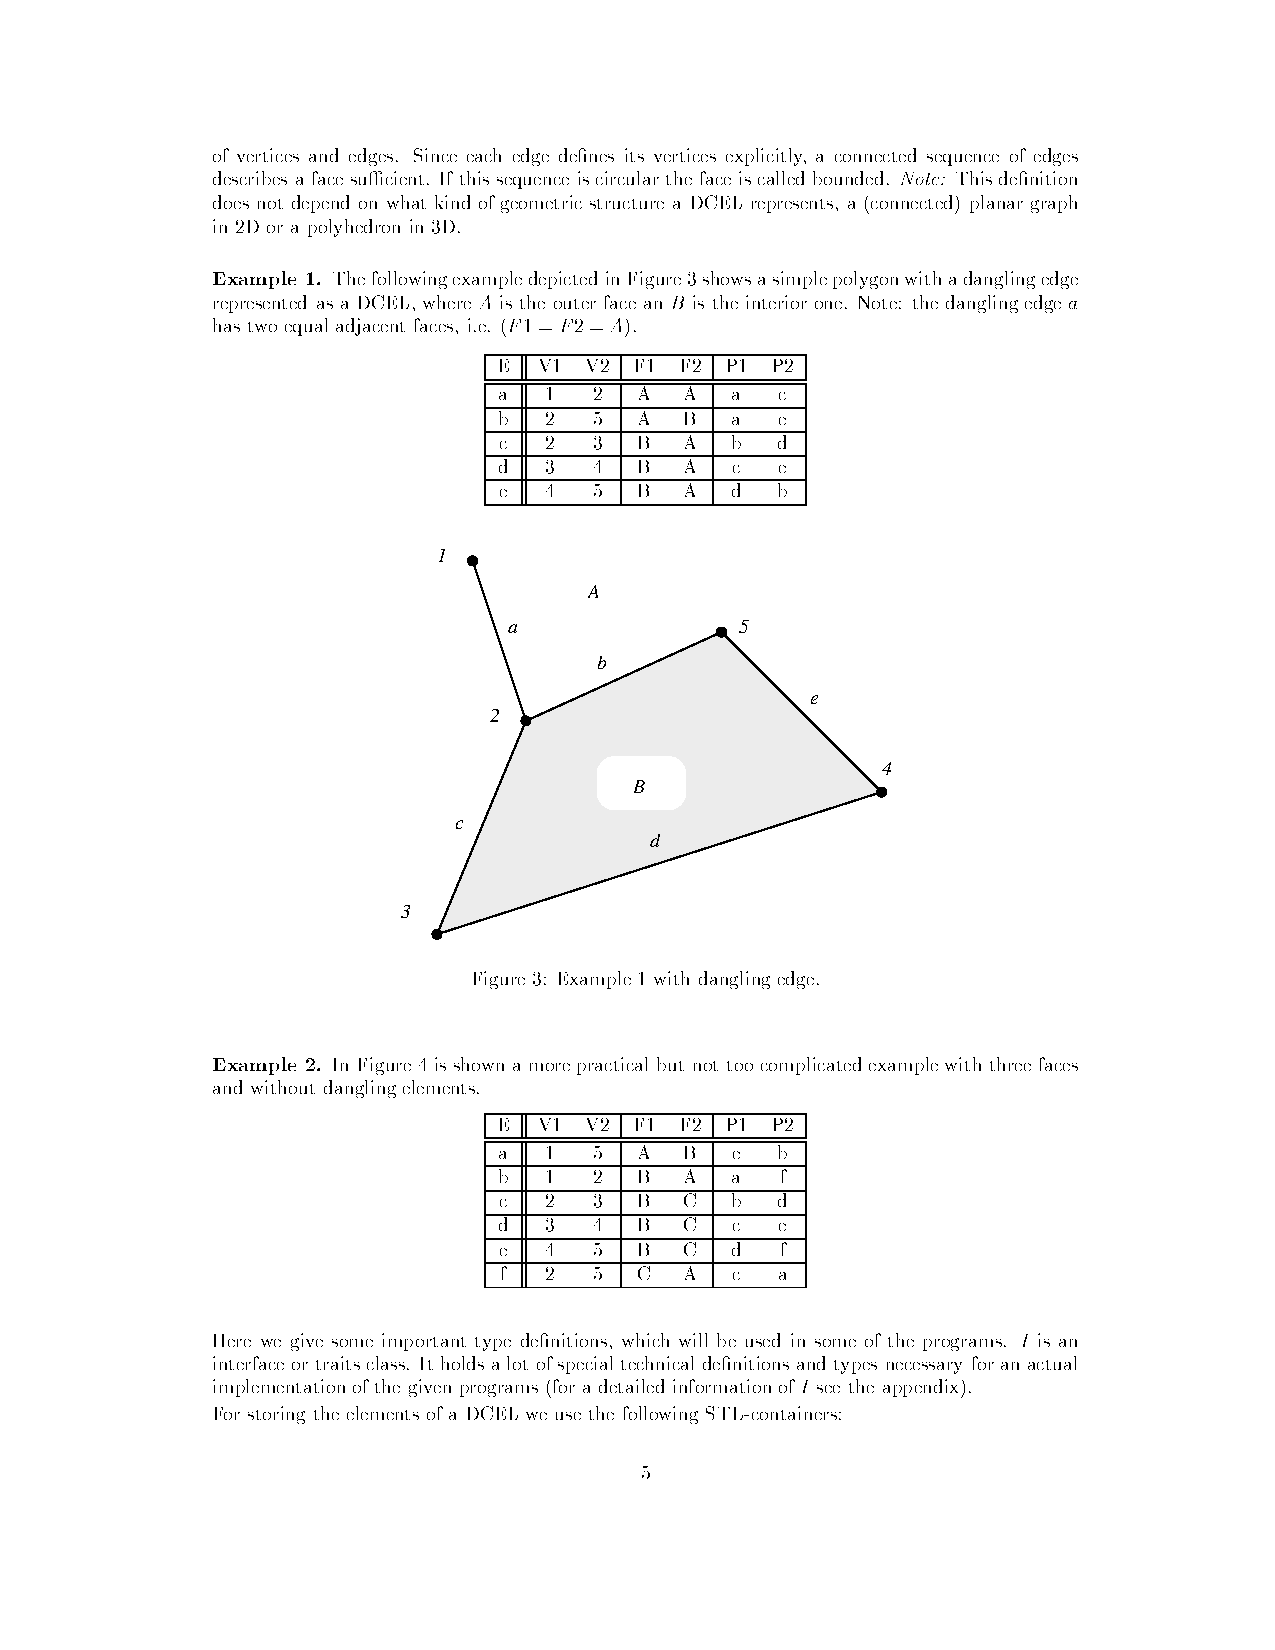
\includegraphics[clip, trim=8cm 19cm 5cm 6cm,width=1.5\linewidth]{figures/dcel02} 
    \end{minipage}
    \flushright \tiny (Freiseisen, 1998)
\end{frame}

\begin{frame}{Computing the overlay}
    \centering 
    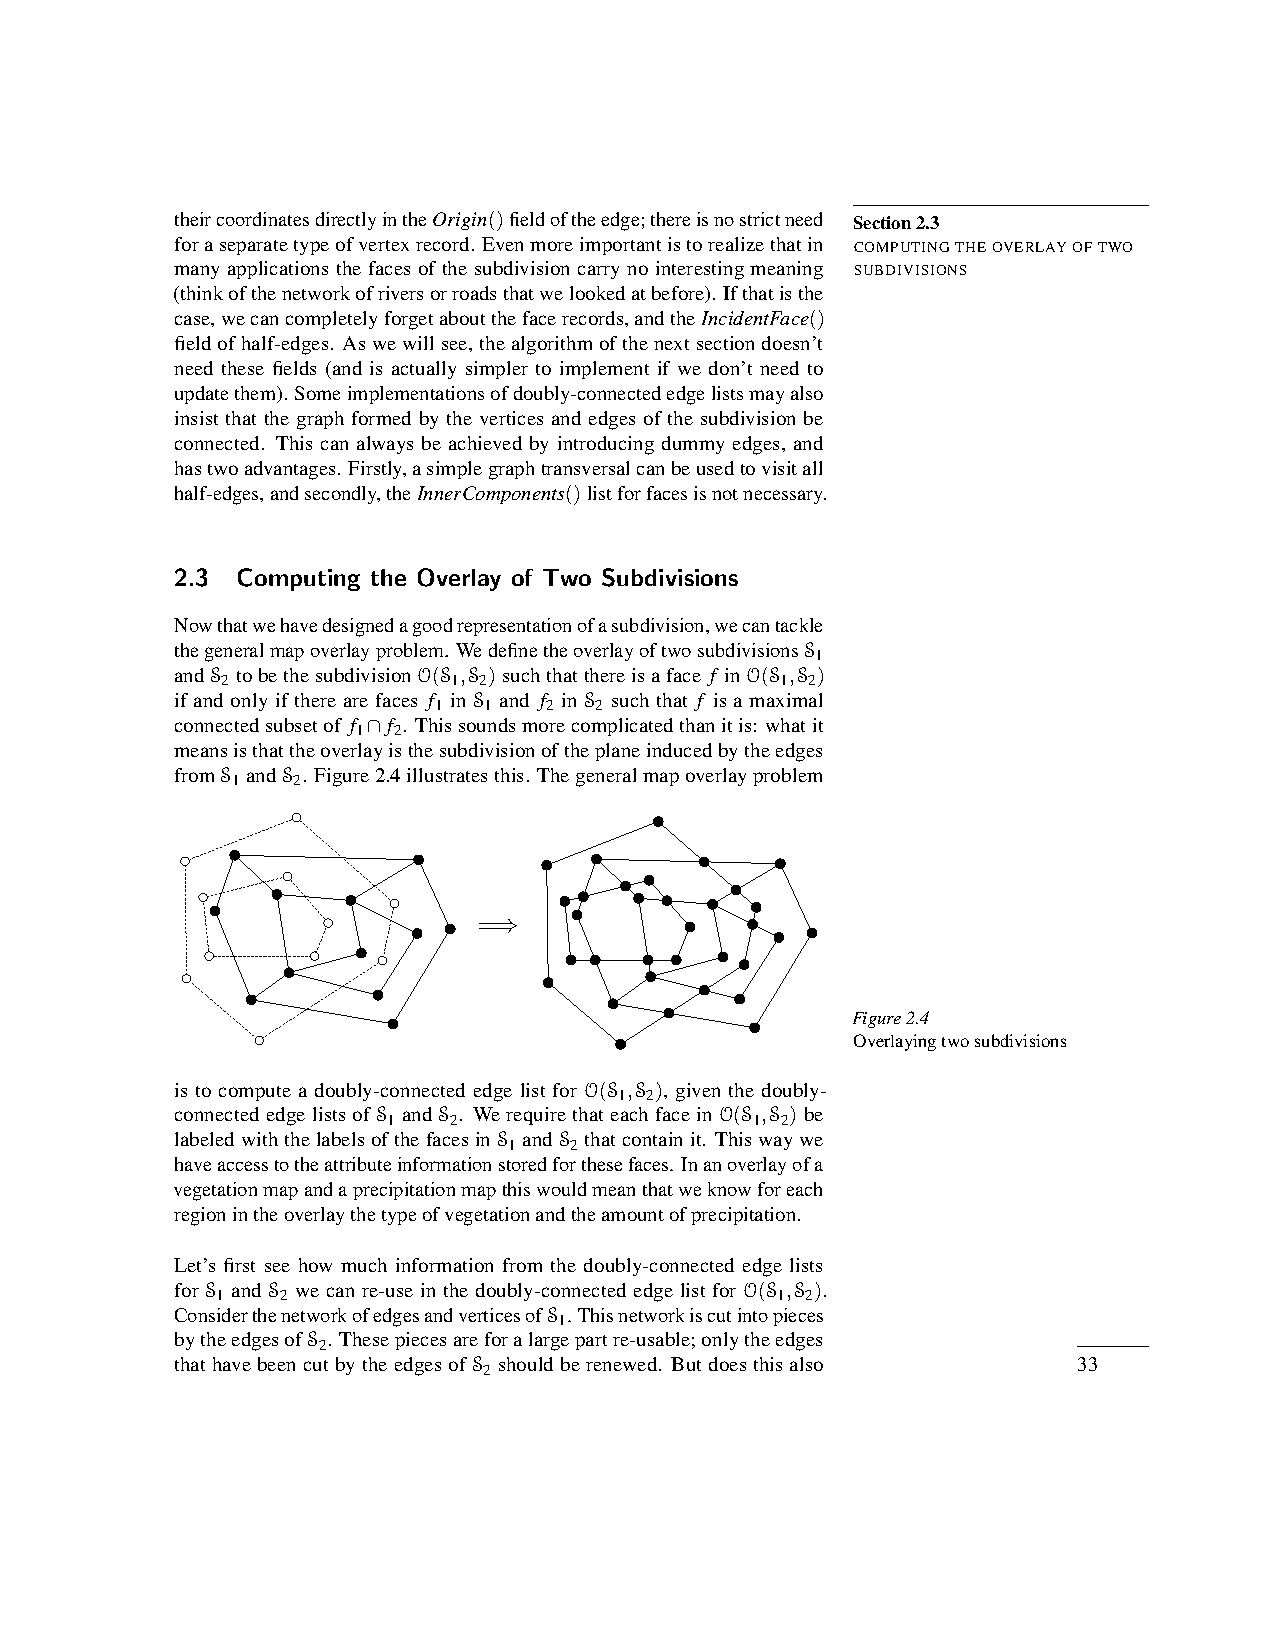
\includegraphics[clip, trim=2cm 10cm 7.5cm 13.5cm,width=\linewidth]{figures/dcel04} 
    \flushright \tiny (de Berg et al, 2008)
\end{frame}

\begin{frame}{The algorithm}
    \begin{enumerate}
        \item Find all intersections over the edges of the polygons.
        \item Construct a planar graph by inserting all edges and all intersections (DCEL).
        \item Traverse this planar graph in order to perform an intersection, union or difference.
    \end{enumerate}
\end{frame}

\begin{frame}{Advantages}
    \begin{itemize}
        \item DCEL captures topological information.
        \item DCEL allows multiple spatial operations.
        \item DCEL can be constructed from this in $\mathcal{O}(n \log(n))$ time using $\mathcal{O}(n)$ additional memory.
        \item DCEL allows boolean operations in $\mathcal{O}(n)$ time using $\mathcal{O}(n)$ additional space.
    \end{itemize}
\end{frame}

\section{Literature review}

\begin{frame}{Literature review}
    \begin{itemize}
        \item A full reference list of relevant papers is available at: \url{http://www.cs.ucr.edu/~acald013/public/RIDIR/R04/DCELReport.html}.
        \item First 5 entries contains solid introductory material about DCELs, specially de Berg et al. (2008) and Freiseisen (1998).
        \item Next entries discuss alternative methods for map overlay, particularly exploring sequential techniques and parallel spatial joins.
        \item \textit{There is no mention to a distributed DCEL implementation.}
    \end{itemize}
\end{frame}

\begin{frame}{Literature review}
    \begin{itemize}
        \item Sequential techniques (more relevant):
        \begin{itemize}
            \item G. Barequet, ``DCEL: A Polyhedral Database and Programming Environment''. IJCGA, vol. 08, pp. 619-636, Oct. 1998.
            \item T. Asano and G. Rote, ``Constant-Working-Space Algorithms for Geometric Problems''. JoCG, vol. 2, pp. 46-68, 2009.
            \item W. Freiseisen, ``Colored DCEL for Boolean Operations in 2D''. Tech report. 1998.
        \end{itemize}
    \end{itemize}
\end{frame}

\begin{frame}{Literature review}
    \begin{itemize}
        \item Parallel spatial joins (more relevant):
        \begin{itemize}
            \item S. Puri and S. K. Prasad, ``Efficient Parallel and Distributed Algorithms for GIS Polygonal Overlay Processing''. Washington, DC, USA, 2013, pp. 2238-2241.
            \item I. Sabek and M. F. Mokbel, ``On Spatial Joins in MapReduce''. 2017, pp. 1-10.
            \item C. Zhou, Z. Chen, and M. Li, ``A parallel method to accelerate spatial operations involving polygon intersections''. IJGIS, vol. 32, no. 12, pp. 2402-2426, Dec. 2018.
            \item W. R. Franklin, S. V. G. de Magalhães, and M. V. A. Andrade, ``Data Structures for Parallel Spatial Algorithms on Large Datasets''. 2018, pp. 16–19.
        \end{itemize}
    \end{itemize}
\end{frame}

\begin{frame}{Current (sequential) implementations}
    \begin{itemize}
        \item CGAL: Computational Geometry Algorithms Library in C++ (binding for Java and Python are available). \url{https://www.cgal.org/}.
        \item dyn4j: A 100\% Java 2D collision detection and physics engine. \url{http://www.dyn4j.org/}.
        \item anglyan/dcel: Python implementation of a doubly connected edge list. \url{https://github.com/anglyan/dcel}.
        \item vpranckaitis/muller-preparata-algorithm: DCEL algorithm implementation and visualisation with Scala. \url{https://github.com/vpranckaitis/muller-preparata-algorithm}.
    \end{itemize}
\end{frame}

\section{Proposal}

\begin{frame}{The proposal}
    \centering
    A parallel DCEL implementation to support big spatial data overlay operations.
\end{frame}

\begin{frame}{What is the problem?}
    \begin{itemize}
        \item Currently, most map overlay methods are sequential based.
        \item For layers with thousand of polygons the execution time is not feasible.
        \item Most of techniques are oriented to a specific spatial operation (intersection, union, difference, ...).
        \item Parallel techniques divide the data into partitions and duplicate features if needed in order to solve the problem locally.
        \item Data structures collecting topological properties are not explored.
    \end{itemize}
%    \centering 
%    \includegraphics[width=.7\linewidth]{p1.png} 
\end{frame}

\begin{frame}{Why is it important?}
    \begin{itemize}
        \item The rise of big (spatial) data makes necesary to count with fast and efficient techniques for spatial analysis.
        \item In particular, the RIDIR project has to deal with spatial operations between layers collecting thousand of counties nation-wide.  The versatility and efficiency of the spatial methods is cardinal for their studies.
        \item It should be interesting to count with intermediate data structures that allow multiple map overlay queries. 
        \item DCEL allows linear time to compute spatial operations.
    \end{itemize}
\end{frame}

\begin{frame}{What are the limitations of related work?}
    \begin{itemize}
        \item Topological data structures are common in computational geometry.  However, most implementations are sequential and they do not scale appropiately on large spatial datasets.
        \item Parallel spatial joins add complexity due to spatial partitioning necessarily introduces replication.
    \end{itemize}
\end{frame}

\begin{frame}{Why is it challenging?}
    \begin{itemize}
        \item Initial stages of the DCEL construction expect it fits in main memory.
        \item Subsequent operations should be able to query the DCEL in a transparent way.
    \end{itemize}
\end{frame}

\begin{frame}{What are our novel contributions?}
    \begin{itemize}
        \item At the best of our knowledge, there is not a distributed DCEL implementation.
        \item It is necesary to design procedures for partitioning and merging during the DCEL construction.
        \item The spatial methods that run over the DCEL are based on boolean operations.  They should be adjusted accordingly to a distributed DCEL.
    \end{itemize}
\end{frame}

\begin{frame}{What is the validation method?}
    \begin{itemize}
        \item We can compare the new implementation to sequential versions of the algorithm.
        \item To test scalability we can perform benchmarks to the current versions of \texttt{area\_tables} and \texttt{area\_interpolate}.
    \end{itemize}
\end{frame}


\end{document}
